\documentclass{article}
\usepackage[utf8]{inputenc}
\usepackage{amssymb}
\usepackage{graphicx}
\usepackage{setspace}
\usepackage{listings}
\usepackage{float}
\usepackage{xcolor}
\usepackage{amsmath}
\usepackage{pgfplots}
\usepackage{enumitem}
\usepackage{subcaption}
\usepackage{hyperref}

\title{\textbf{High Performance Computer Architectures Practical Course \\ - Exercise 4 -} \\[10mm]}
\author{Tutorium 1 \\[10mm] David Jordan (6260776) \\[1mm] Florian Rüffer (7454628) \\[1mm] Michael Samjatin (7485765) \\[10mm]}


\lstset{
    language=C++,
    basicstyle=\ttfamily,
    keywordstyle=\color{blue},
    stringstyle=\color{red},
    commentstyle=\color{green},
    numbers=left,
    numberstyle=\normalsize,
    breaklines=true,
    showstringspaces=false,
    frame=single,
    linewidth=1\linewidth,
    captionpos=b
}
\renewcommand{\lstlistingname}{File}% Listing -> Algorithm
\renewcommand{\lstlistlistingname}{List of \lstlistingname s}% List of Listings -> List of Algorithms

\begin{document}
\maketitle
\newpage
\section{Matrix}
\section{Quadratic Equation}
\section{Newton}
In this task we have to vectorize the Newton method. As mentioned in the task description
the Newton Method is an interative process to approximate the x-axis intersection. \\[5mm]

\begin{lstlisting}[caption=Newton.cpp]
    float_v FindRootVector(const float_v& p1, const float_v& p2)
    {
      float_v x = 1.f, x_new = 0.f;
      float_m mask(true);
      for( ; !mask.isEmpty(); ) {
          // for(int i = 0; i < 1000; ++i){ 
        x = x_new;
        x_new(mask) = x - F(x,p1,p2) / Fd(x,p1,p2);
        mask = abs((x_new - x)/x_new) > P;
      }
      return x_new;
    }
\end{lstlisting}

\noindent The main idea of vectorizing the Newton method, is the calculation of multiple roots at once.
This comes along with an issue, because if multiple roots are calculate, then also some of those will
reach the desired precision earlier than others. To solve this problem we will use masks.
The underlying principle of masks is a vector with each value mapped to a boolean.
Each boolean value corresponds to the value of another vector.
Using this methodology we can assign 'false' to a corresponding number, which already has our desired precision and therefore
exclude it from further unneccessary calculations.\\

\noindent The first iteration will start with a mask of only 'true' values, as no value has yet reached the desired precision.
This means every value will be updated accordingly with $x - F (x , p1 , p2 ) / Fd (x , p1 , p2 ) $.
The next iteration will only update those values, which need further refinement ($\rightarrow$ mask value equals 'true') with $mask = abs (( x_new - x ) / x_new ) > P $.

\begin{figure}[H]
    \begin{center}
        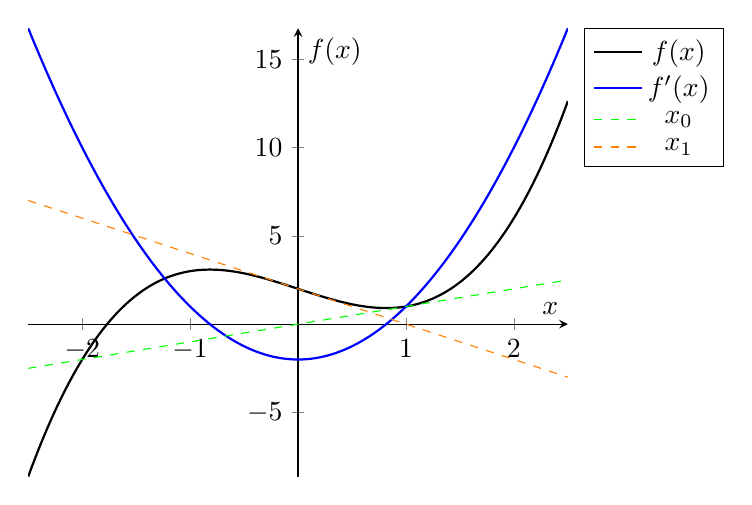
\begin{tikzpicture}[
            declare function={
                func(\x)= \x^3 - 2*\x + 2;
                derivative(\x) = 3*\x^2 - 2;
            }
        ]
        \begin{axis}[
            axis lines=middle,
            xlabel=$x$,
            ylabel={$f(x)$},
            domain=-2.5:2.5,
            samples=200,
            legend pos=outer north east
        ]
        \addplot [thick, black, smooth] {func(x)};
        \addlegendentry{$f(x)$}
        \addplot [thick, blue, smooth] {derivative(x)};
        \addlegendentry{$f'(x)$}
        
        \pgfmathsetmacro{\a}{1}
        \pgfmathsetmacro{\b}{\a - func(\a)/derivative(\a)}
        
        \addplot [green, dashed, samples=2, domain=(-2.5:2.5)] {(func(\a) + derivative(\a) * (x - \a))};
        \addlegendentry{$x_0$}
        
        \pgfmathsetmacro{\a}{\b}
        \pgfmathsetmacro{\b}{\a - func(\a)/derivative(\a)}
        
        \addplot [orange, dashed, samples=2, domain=(-2.5:2.5)] {(func(\a) + derivative(\a) * (x - \a))};
        \addlegendentry{$x_1$}
        
        \pgfmathsetmacro{\a}{\b}
        \pgfmathsetmacro{\b}{\a - func(\a)/derivative(\a)}
        
        \end{axis}
        \end{tikzpicture}
    \end{center}   
\end{figure}

\section{Random Access}

\begin{figure}[H]
    \centering
    \includegraphics[scale=0.5]{example-image.png} 
    \caption{Output}
    \label{fig:example}
\end{figure}







\end{document}
